% Selected v0.5 Candidate B, unchanged from main 9014e4b after PR #24.
\begin{figure*}[t]
\centering
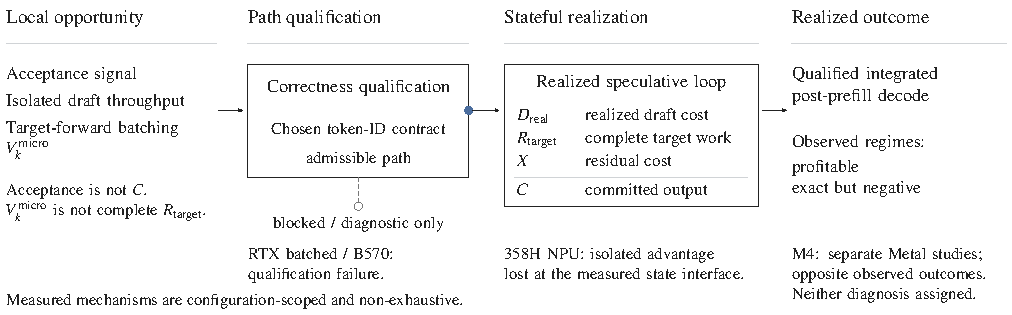
\includegraphics[width=\textwidth]{../figures/mechanism_v05/mechanism.pdf}
\caption{\textbf{From local opportunity to integrated post-prefill decode outcomes.} Local acceptance, isolated drafting, and target-forward batching do not by themselves establish integrated gains. Arrows mark evaluation boundaries, not a guarantee of gain. The frozen greedy token-ID contract excludes the tested RTX 5070 Ti Laptop batched path; B570 serialization improves agreement without qualifying the full workload. Blocked timings remain diagnostic. For the qualified 358H NPU path, full-prefix replay and proposal share one synchronous OpenVINO call, and the isolated draft advantage does not survive the tested stateful integration. $D_{\mathrm{real}}$, $R_{\mathrm{target}}$, and $X$ normalize measured draft, complete target, and residual costs by matched target-only token cost; $C$ counts all committed output, including correction/bonus tokens. M4\textquotesingle s separate frozen studies on the same tested Metal stack yield opposite exact regimes. Workload and session conditions differ, and neither diagnosis is assigned to the contrast. The measured mechanisms are configuration-scoped and non-exhaustive; timing excludes loading and initial prompt prefill.}
\label{fig:translation}
\end{figure*}
